\chapter{Epoch Boundary Blocks}
\label{ebbs}

\section{Introduction}

Recall that when a new epoch begins, the active stake distribution in the new
epoch---that is, the stake distribution used to determine the leader schedule---
is not the stake distribution as it was at the end of the last epoch, but
rather as it was some distance back:
%
\begin{center}
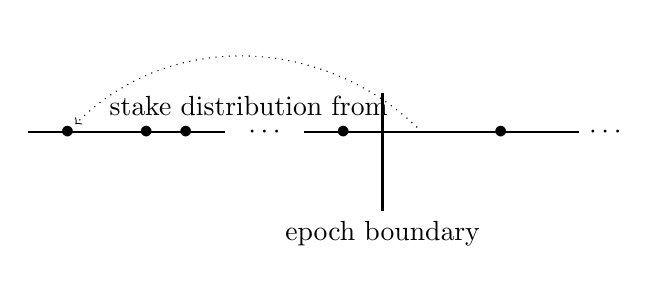
\begin{tikzpicture}
\draw
     (0   , 0)
  -- (0.5 , 0) node{$\bullet$}
  -- (1.5 , 0) node{$\bullet$}
  -- (2   , 0) node{$\bullet$}
  -- (2.5 , 0);
\node at (3,0) {$\cdots$};
\draw
     (3.5 , 0)
  -- (4   , 0) node{$\bullet$}
  -- (6   , 0) node{$\bullet$}
  -- (7   , 0) node[right]{$\cdots$};
\draw [very thick] (4.5,0.5) -- (4.5,-1) node[below] {epoch boundary};
\draw [->, dotted] (5,0) to [out=135,in=45] (0.6,0.1);
\path (5,0) -- (0.6,0.1) node[pos=0.5,above=1] {stake distribution from};
\end{tikzpicture}
\end{center}
%
This means that blocks cannot influence the active stake distribution until
some time in the future. That is important, because when a malicious node
forks off from the honest chain, the leadership schedule near the intersection
point cannot be influenced by the attacker, allowing us to compare chain
density and choose the honest chain (which will be denser because of the
assumed honest majority); see \cref{genesis} for an in-depth discussion.

In the literature, the term ``epoch boundary block'' (or EBB for short) normally
simply refers to the last block in any given epoch (for example,
see~\cite{buterin2020combining}). It might therefore be a bit surprising to find
the term in this report since the final block in an epoch is not of special
interest in the Ouroboros family of consensus protocols. However, in the first
implementation of the Byron ledger (using the original Ouroboros protocol
\cite{cryptoeprint:2016:889}, which we now refer to as ``Ouroboros Classic''), a
decision was made to include the leadership schedule for each new epoch as an
explicit block on the blockchain; the term EBB was used to refer to this special
kind of block:\footnote{It is not entirely clear if an EBB should be regarded as
the final block in an epoch, or as the first block in the next epoch. The name
would suggest that the former interpretation is more appropriate; as it turns
out, however, the very first epoch on the chain \emph{starts} with an EBB,
recording the leadership schedule derived from the genesis block. We will
therefore regard the EBB as starting an epoch, rather than ending one.}
%
\begin{center}
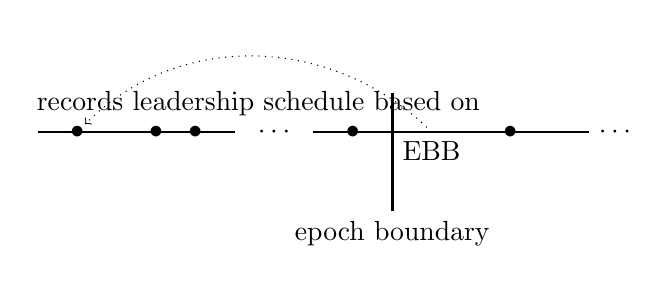
\begin{tikzpicture}
\draw
     (0   , 0)
  -- (0.5 , 0) node{$\bullet$}
  -- (1.5 , 0) node{$\bullet$}
  -- (2   , 0) node{$\bullet$}
  -- (2.5 , 0);
\node at (3,0) {$\cdots$};
\draw
     (3.5 , 0)
  -- (4   , 0) node{$\bullet$}
  -- (6   , 0) node{$\bullet$}
  -- (7   , 0) node[right]{$\cdots$};
\draw [very thick] (4.5,0.5) -- (4.5,-1) node[below] {epoch boundary};
\draw [->, dotted] (5,0) to [out=135,in=45] (0.6,0.1);
\path (5,0) -- (0.6,0.1) node[pos=0.5,above=1] {records leadership schedule based on};
\node at (5,0) {$\blacksquare$};
\node [below=0.1] at (5,0) {EBB};
\end{tikzpicture}
\end{center}

Having the leadership schedule explicitly recorded on-chain turns out not to
be particularly useful, however, and the code was modified not to produce EBBs
anymore even before we switched from Byron to Shelley (as part of the OBFT hard
fork, see \cref{overview:history}); these days, the contents of the existing
EBBs on the chain are entirely ignored. Unfortunately, we cannot forget about
EBBs altogether because---since they are an actual block on the
blockchain---they affect the chain of block hashes: the first ``real'' block in
each epoch points to the EBB as its predecessor, which then in turns points to
the final block in the previous epoch.

So far, none of this is particularly problematic to the consensus layer. Having
multiple types of blocks in a ledger presents some challenges for serialisation
(\cref{serialisation:storage:nested-contents}), but does not otherwise affect
consensus much: after all, blocks are interpreted by the ledger layer, not by
the consensus layer. Unfortunately, however, the design of the Byron EBBs has
odd quirk: an EBB has the same block number as its \emph{predecessor}, and the
same slot number as its \emph{successor}:
%
\begin{center}
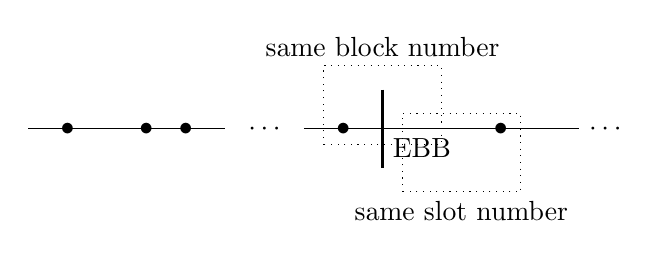
\begin{tikzpicture}
\draw
     (0   , 0)
  -- (0.5 , 0) node{$\bullet$}
  -- (1.5 , 0) node{$\bullet$}
  -- (2   , 0) node{$\bullet$}
  -- (2.5 , 0);
\node at (3,0) {$\cdots$};
\draw
     (3.5 , 0)
  -- (4   , 0) node{$\bullet$}
  -- (6   , 0) node{$\bullet$}
  -- (7   , 0) node[right]{$\cdots$};
\draw [very thick] (4.5,0.5) -- (4.5,-0.5);
\node at (5,0) {$\blacksquare$};
\node [below=0.1] at (5,0) {EBB};
%
\draw [dotted]
     (3.75, -0.2)
  -- ++(0, 1)
  -- ++(1.5, 0) node[pos=0.5,above] {same block number}
  -- ++(0, -1)
  -- cycle;
\draw [dotted]
     (4.75, -0.8)
  -- ++(0, 1)
  -- ++(1.5, 0)
  -- ++(0, -1)
  -- cycle  node[pos=0.5,below] {same slot number};
\end{tikzpicture}
\end{center}
%
This turns out to be a huge headache. When we started the rewrite, I think we
underestimated quite how many parts of the system would be affected by the
possibility of having multiple blocks with the same block number and
multiple blocks with the same slot number on a single chain. Some examples
include:

\begin{itemize}
\item \label{ebb-chain-selection}
For chain selection protocols based on chain length, two chains may end in
blocks with the same block number, yet not have equal length.

\item When we validate block headers that contain explicit block numbers, we
cannot insist that those block numbers are monotonically increasing, instead
having to add a special case for EBBs.

\item TODO: Many, many others
\end{itemize}

In hindsight, we should have tried harder to eliminate EBBs from the get-go. In
this chapter, we will discuss two options for modifying the existing design to
reduce the impact of EBBs (\cref{ebbs:logical}), or indeed eliminate them
altogether (\cref{ebbs:elimination}).

\section{Logical slot/block numbers}
\label{ebbs:logical}

\section{Eliminating EBBs altogether}
\label{ebbs:elimination}









% For the Ouroboros family of consensus
% protocols, the last block in an epoch is not of special interest, so it
% might be surprising to see the term EBB in this report.
%
% When a new epoch
% begins---that is, at an epoch boundary---the active stake distribution shifts,
% but it is not based on the final block in the previous epoch, but instead on
% the ledger state as it was quite a bit earlier. As a consequence, blocks cannot
% have an effect on the leadership schedule until they are a certain depth into
% the chain. This is important, because it means that if there is a fork in the
% chain, the leadership schedule after the intersection point will be determined
% by the common prefix of both chains.


%
%
% section 3 (The Ouroboros Protocol)
%
% Stage 1: "There is an initial stake distribution which is hardcoded into the genesis block"


% Discuss that although EBBs are a Byron concern, their presence has far reaching
% consequences on the consensus later. In hindsight, we should have tried harder
% to not deal with them at all from the beginning; we did not anticipate quite how
% bad the situation would be. We now have a plan for getting rid of them
% (\cref{decontamination-plan}) but it will be a fairly long term thing and it
% might not happen at all, depending on quite how much time is available for
% removing tech debt.
%
%
% \section{Introduction}
%
% \section{Consequences}
%
% \subsection{Chain selection}
% \label{ebb-chain-selection}
%
% \section{Elimination}
% \label{decontamination-plan}
